\documentclass[12pt, a4paper]{article}

% --- Pacotes Básicos ---
\usepackage[utf8]{inputenc}
\usepackage[T1]{fontenc}
\usepackage[brazil]{babel}
\usepackage{geometry}
\geometry{a4paper, margin=2.5cm}
\usepackage{graphicx} % Para inserir os prints da tela
\usepackage{float}    % Para forçar o posicionamento das imagens
\usepackage{booktabs} % Para tabelas mais bonitas
\usepackage{hyperref} % Para links clicáveis no sumário
\usepackage{listings} % Para inserir trechos de código (se necessário)
\usepackage{xcolor}

% --- Configuração de Cores para o Código ---
\definecolor{codegreen}{rgb}{0,0.6,0}
\definecolor{codegray}{rgb}{0.5,0.5,0.5}
\definecolor{codepurple}{rgb}{0.58,0,0.82}
\definecolor{backcolour}{rgb}{0.95,0.95,0.92}

\lstdefinestyle{mystyle}{
    backgroundcolor=\color{backcolour},   
    commentstyle=\color{codegreen},
    keywordstyle=\color{magenta},
    numberstyle=\tiny\color{codegray},
    stringstyle=\color{codepurple},
    basicstyle=\ttfamily\footnotesize,
    breakatwhitespace=false,         
    breaklines=true,                 
    captionpos=b,                    
    keepspaces=true,                 
    numbers=left,                    
    numbersep=5pt,                  
    showspaces=false,                
    showstringspaces=false,
    showtabs=false,                  
    tabsize=2
}
\lstset{style=mystyle}

% --- Informações do Documento ---
\title{\textbf{Relatório Prático: Cálculo de Números Primos com OpenMP}\\
\large Laboratório de Programação Paralela}
\author{
    Eduardo Rottschaefer Oliveira\\
}
\date{\today}

\begin{document}

\maketitle

\tableofcontents
\newpage

% --- 1. Introdução ---
\section{Introdução}
Este relatório descreve a implementação, execução e análise de desempenho de programas para o cálculo de números primos até o limite de $N = 500.000.000$. O objetivo principal é analisar o comportamento de diferentes políticas de escalonamento em ambientes de memória compartilhada utilizando OpenMP.

Dois algoritmos base foram utilizados: uma abordagem \textit{Naive} (Ingênua) e uma abordagem Otimizada (\textit{Bag of Tasks}).

% --- 2. Metodologia ---
\section{Metodologia e Ambiente de Testes}
As execuções seguiram estritamente os parâmetros estabelecidos para o experimento:
\begin{itemize}
    \item \textbf{Valor Limite ($N$):} 500.000.000
    \item \textbf{Número de Threads:} 4
    \item \textbf{Tamanho do Chunk:} 10
    \item \textbf{Políticas Avaliadas:} \texttt{static}, \texttt{dynamic} e \texttt{guided}.
\end{itemize}

O ambiente de execução (hardware e sistema operacional) utilizado para coletar os tempos foi:
\begin{itemize}
    \item \textbf{Processador:} 11th Gen Intel® Core™ i3-1115G4 × 4
    \item \textbf{Memória RAM:} 8 GB
    \item \textbf{Sistema Operacional:} Ubuntu 24.04.1 LTS
\end{itemize}

% --- 3. Abordagens Algorítmicas ---
\section{Abordagens Algorítmicas}
Nesta seção, detalhamos brevemente a lógica das duas abordagens implementadas para evidenciar o impacto no balanceamento de carga entre as threads.

O Algoritmo aplicado itera por todos os números até a raiz quadrada de $n$, eliminando previamente os números pares.


\subsection{Algoritmo Naive (Ingênuo)}

Foi utilizado o escalonamento \texttt{static}, onde o conjunto dos N números foi dividido em pedaços (chunks) de tamanho 10 e cada thread sabe antes da execução do laço quais pedaços vai executar.

\subsection{Algoritmo Otimizado (Bag of Tasks nativo)}
Existem duas técnicas de escalonamento que simulam o comportamento de um \textit{Bag of Tasks}. O primeiro é o \texttt{dynamic} que provê pedaços (chunks) de 10 iterações sob demanda para as threads ociosas.

O segundo é o \texttt{guided}, onde o tamanho do chunk também é 10, com a diferença de que o chunck definido limita o tamanho mínimo do pedaço de iterações que será provido a cada thread, podendo esse ser maior. Aqui a divisão de trabalho entre threads também é feita durante a execução do laço, distribuindo pedaços do laço dinamicamente para as thread ociosas.

% --- 4. Resultados e Prints ---
\section{Resultados e Execuções (Prints)}
Abaixo estão registradas as capturas de tela (\textit{prints}) demonstrando as execuções de cada modo de escalonamento.

% EXEMPLO DE COMO INSERIR A IMAGEM
% Descomente as linhas abaixo e troque 'nome_da_imagem.png' pelo arquivo real que você subir no Overleaf

\begin{figure}[H]
    \centering
    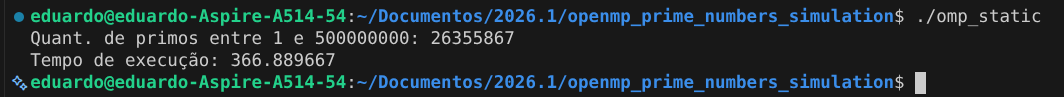
\includegraphics[width=0.8\textwidth]{naive_static.png}
    \caption{Execução 1: Algoritmo com Escalonamento Static.}
    \label{fig:naive_static}
\end{figure}

\begin{figure}[H]
    \centering
    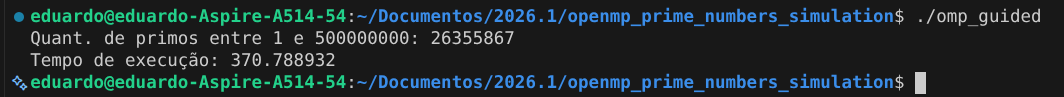
\includegraphics[width=0.8\textwidth]{naive_guided.png}
    \caption{Execução 2: Algoritmo com Escalonamento Guided.}
    \label{fig:naive_guided}
\end{figure}

\begin{figure}[H]
    \centering
    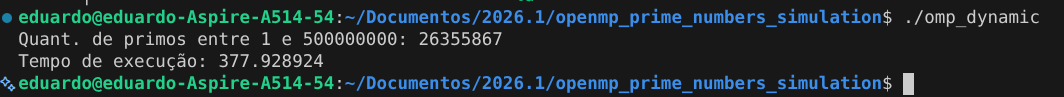
\includegraphics[width=0.8\textwidth]{bag_of_tasks.png}
    \caption{Execução 3: Algoritmo com Escalonamento Dynamic (Bag of Tasks).}
    \label{fig:bag_dynamic}
\end{figure}


% --- 5. Análise de Desempenho ---
\section{Análise de Desempenho}
Os tempos de execução coletados via \texttt{omp\_get\_wtime()} foram consolidados na Tabela \ref{tab:resultados}.

\begin{table}[H]
    \centering
    \begin{tabular}{@{}llc@{}}
        \toprule
        \textbf{Algoritmo} & \textbf{Escalonamento (Chunk 10)} & \textbf{Tempo de Execução (s)} \\ \midrule
        Naive             & Static                            & 366.89                        \\
        Bag of Tasks             & Guided                            & 370.79                        \\ 
        Bag of Tasks   & Dynamic                           & 377.93                       \\
  \bottomrule
    \end{tabular}
    \caption{Comparativo de tempos de execução (N=500.000.000, 4 Threads)}
    \label{tab:resultados}
\end{table}

\subsection{Discussão dos Resultados}
    Vimos um melhor desempenho do escalonamento \texttt{static} perante às outras opções. Isso se deve ao fato de que o overhead de processamento ao distribuir a computação para as threads é menor, já que isso é definido antes do laço executar. 
    
    Com escalonamento \texttt{dynamic} e \texttt{guided}, as threads ainda não sabem qual é o próximo chunk a ser executado por elas, por isso precisam pedir essa informação para a thread master. Dependendo do contexto, isso pode ser válido para balancear melhor a carga de computação entre as threads, mesmo que exista o overhead de distribuição de trabalho. No nosso caso, o overhead de distribuição foi maior que o ganho com o balanceamento de carga, visto o pior desempenho.

    O escalonamento \texttt{guided} ainda obteve um desempenho melhor que o \texttt{dynamic}. Este divide todo bloco em chuncks de tamanho exatamente igual a 10, enquanto o \texttt{guided} tem chuncks de tamanhos maiores no início, o que gera menos blocos de computação a serem distribuidos. Logo, considerando o maior trabalho de distribuição que o \texttt{dynamic} tem pela quantidade de blocos a distribuir, o overhead dessa técnica de escalonamento foi pior nesse caso.


% --- 6. Conclusão ---
\section{Conclusão}
A experimentação prática validou de forma empírica os conceitos de balanceamento de carga e paralelismo de loop em OpenMP. Fica evidente que, mesmo que mais simples, o escalonamento \texttt{static} pode ser uma melhor opção, dependendo do contexto onde é utilizado. Não existe bala de prata, é preciso uma análise detalhada de cada problema para que se decida o tipo de escalonamento a se utilizar.

\end{document}